% !TEX root = ../thesis-example.tex
%
\chapter{Proponowane algorytmy}
\label{sec:proponowane_algorytmy}

Niniejszy rozdział opisuje szczegółowo kolejne kroki rozwiązania problemu, który został dokładnie przestawiony w sekcji \ref{sec:wstep:opis_problemu}. Sekcja \ref{sec:proponowane_algorytmy:oprogramowanie} opisuje sposób implementacji oprogramowania oraz wykorzystane technologie. Sekcja \ref{sec:proponowane_algorytmy:wiedza_dziedzinowa} opisuje wiedzę dziedzinową na temat danych wejściowych (kafelków). Następnie sekcje od \ref{sec:proponowane_algorytmy:sift} do \ref{sec:proponowane_algorytmy:laczenie_kafelkow} opisują zasadę działania poszczególnych metod w kolejności zgodnej z ich wykonywaniem w programie.

\section{Oprogramowanie}
\label{sec:proponowane_algorytmy:oprogramowanie}

Program o nazwie \texttt{mostitch}, który jest celem niniejszej pracy jest całkowicie napisany w języku C++. Ten język został wybrany ze względu na to, że wykorzystywana biblioteka przetwarzania obrazów OpenCV (opisana w skrócie w sekcji \ref{sec:proponowane_algorytmy:opencv}) posiada interfejs w języku C++. Program można uruchomić z konsoli systemu za pomocą komendy:

\begin{verbatim}
./mostitch path_to_config_file
\end{verbatim}

gdzie \texttt{path\_to\_config\_file} to obowiązkowy argument do programu, który wskazuję ścieżkę do pliku konfiguracyjnego (opisanego dokładniej w sekcji \ref{sec:proponowane_algorytmy:plik_configuracyjny}), który określa wszystkie parametry niezbędne do prawidłowego działania programu.

Program umożliwia stworzenie mozaik dla dowolnej ilości zbiorów kafelków. Dodatkowo dla każdego zbioru kafelków powstają różne wersje mozaik, ze względu na wykorzystanie różnych metod ich tworzenia. Dzięki tej funkcjonalności użytkownik może wybrać mozaikę, która jest najbardziej odpowiednia. Wyjściem programu więc jest zbiór mozaik (obrazy \texttt{.png}), w których każdy z nich odpowiada wybranemu zbioru kafelków oraz metodzie tworzenia.

\subsection{Plik konfiguracyjny}
\label{sec:proponowane_algorytmy:plik_configuracyjny}

Do zarządzania plikiem konfiguracyjnym została wykorzystana biblioteka \textbf{libconfig}\footnote{\url{http://www.hyperrealm.com/libconfig/}}, która umożliwia bezproblemowy odczyt pliku konfiguracyjnego z rozszerzeniem \texttt{.cfg}. Format pliku konfiguracyjnego jest bardziej czytelny w porównaniu do powszechnie wykorzystywanych plików XML. Biblioteka również jest świadoma typu zmiennej przez co unika się konwersji typu \texttt{string} na typy takie jak \texttt{int}, czy \texttt{float}.

W pliku konfiguracyjnym zawarte są informacje:

\begin{itemize}
\item Ścieżka do folderu z folderami zawierającymi zbiory kafelków do złączenia.
\item Ścieżka do miejsca, w którym będą zapisane wynikowe mozaiki.
\item Parametry pozwalające na automatyczne wczytanie obrazów kafelków.
\item Parametry modyfikujące działanie metod przetwarzania kafelków.
\end{itemize}

Wszystkie parametry zawarte w pliku konfiguracyjnym są szczegółowo opisane w przykładzie pliku konfiguracyjnego o nazwie \texttt{config.cfg}, który jest dołączony do niniejszej pracy.

\subsection{OpenCV}
\label{sec:proponowane_algorytmy:opencv}

Wszystkie rozwiązania zaimplementowane w niniejszej pracy bazują na bibliotece przetwarzania obrazów o nazwie \textbf{OpenCV}. Biblioteka jest dozwolona do bezpłatnego wykorzystania w projektach prywatnych i komercyjnych. OpenCV jest używane w ogromnej ilości projektów z różnych dziedzin i została ściągnięta już ponad 9 milionów razy\footnote{\url{http://opencv.org}}. OpenCV cieszy się taką popularnością ze względu na szybkość działania, implementację większości metod przetwarzania obrazu oraz umiejętnością pracy na wielu rdzeniach. Kod źródłowy biblioteki jest dostępny publicznie w serwisie Github\footnote{\url{https://github.com/Itseez/opencv}} przez co każdy może rozwijać OpenCV i ma wgląd do zaimplementowanych metod.

\section{Wiedza dziedzinowa}
\label{sec:proponowane_algorytmy:wiedza_dziedzinowa}

Wiedza dziedzinowa określa zbiór informacji związanych z problemem i danymi wejściowymi. Dokładne zdefiniowanie oraz analiza wiedzy dziedzinowej prowadzi do ułatwienia problemu oraz lepszych rezultatów. W przypadku problemu niniejszej pracy danymi wejściowymi do stworzenia mozaiki są angiograficzne obrazy OCT (kafelki). Są to monochromatyczne obrazy o rozmiarze 240 na 240 pikseli. Wraz z obrazami do programu dostarczane są jeszcze dwie informacje:

\begin{itemize}
\item Względna pozycja kafelków względem siebie, która jest zapisana w nazwie obrazu. Lokalizacja jest podana za pomocą współrzędnych x i y układu kartezjańskiego.
\item Szacowany obszar nałożenia kafelków na siebie wyrażony w procentach szerokości obrazu.
\end{itemize}

Na rysunku \ref{fig:proponowane_algorytmy:example} jest przedstawiony przykładowy zbiór kafelków przeznaczony do stworzenia jednej mozaiki wraz z dostarczoną wiedzą dziedzinową.

\begin{figure}[H]
  \centering
  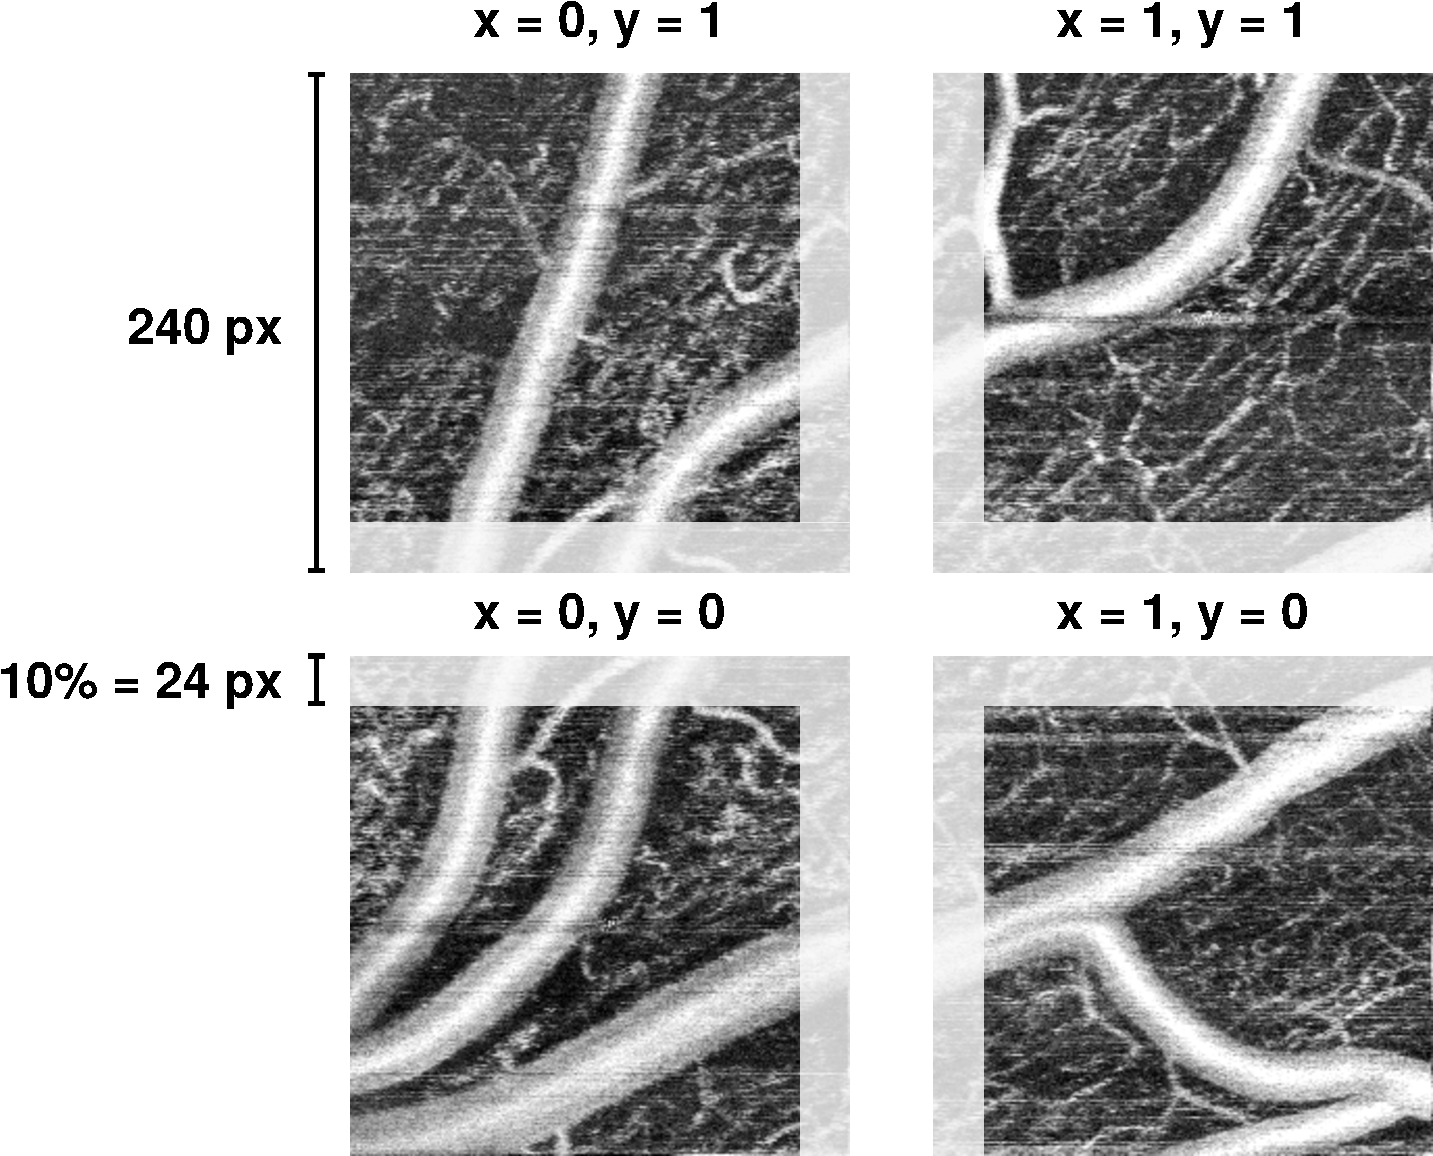
\includegraphics[width=\textwidth]{gfx/example}
  \caption{Cztery kafelki rozmieszone zgodnie z ich pozycją w docelowej mozaice. Na każdym obrazie białym przeźroczystym prostokątem zaznaczony jest oszacowany obszar nałożenia sąsiadujących kafelków.}
  \label{fig:proponowane_algorytmy:example}
\end{figure}

Informacje dostarczone wraz z kafelkami mają istotny wpływ na działanie algorytmu. Jasno podane położenie kafelek informuje algorytm, który kafelek należy dopasowywać z którym (sekcja \ref{sec:proponowane_algorytmy:filtrowanie}), a szacowany obszar nałożenia określa obszar, w którym należy ekstrahować cechy (sekcja \ref{sec:proponowane_algorytmy:sift}). Bez tych informacji stworzenie mozaiki byłoby o wiele bardziej skomplikowane.

\section{Rejestracja kafelków z wykorzystaniem cech}
\label{sec:proponowane_algorytmy:cechy}

Idea ekstrakcji cech w celu rejestracji obrazów została opisana w sekcji \ref{sec:algorytmy_korejestracji:korejestracja_na_podstawie_cech} i jest to pierwszy krok w tworzeniu mozaiki. W niniejszej sekcji najpierw zostanie wyjaśniony wybrany algorytm do ekstrakcji cech oraz sposób jego użycia w programie (sekcja \ref{sec:proponowane_algorytmy:sift}). Następnie przedstawiony zostanie proces dopasowania wyekstrahowanych cech do siebie (sekcja \ref{sec:proponowane_algorytmy:dopasowanie}), a na koniec tej sekcji wyjaśnione zostanie filtrowanie znalezionych dopasowań (sekcja \ref{sec:proponowane_algorytmy:filtrowanie}).

\subsection{Algorytm SIFT}
\label{sec:proponowane_algorytmy:sift}

\textbf{SIFT} (ang. \textit{scale-invariant feature transform}) to algorytm służący do wykrycia i opisania cech w obrazie. Został opublikowany przez David Lowe w 1999 roku \cite{Lowe:2004:DIF:993451.996342}. Dzięki umiejętności wyekstrahowania cech, które są niewrażliwe na rotacje, skalowanie, lokalizacje i przekształcenie afiniczne obrazu jest stosowany w wielu aplikacjach (np. lokalizacja robota \cite{conf/icra/2001}, czy rozpoznawanie zachowań człowieka \cite{Laptev:2007:LVM:1314710.1314906}).

Działanie algorytmu można podzielić na 6 kroków, które są opisane w kolejności wykonania poniżej.

\subsubsection{1. Reprezentacja obszaru za pomocą przestrzeni \textit{scale-space}}
\label{sec:proponowane_algorytmy:scale_space}

Algorytm rozpoczyna swoją pracę tworząc przestrzeń \textit{scale-space} obszaru obrazu, w którym ma wyekstrahować cechy. \textit{Scale-space} generuje się poprzez kilkakrotne użycie filtru Gaussa z różną siłą na docelowym obszarze. Następnie oryginalny obraz próbkujemy zmniejszając jego wielkość dwukrotnie i powtarzamy proces użycia filtru Gaussa. Obrazy o tej samej wielkości tworzą oktawę. Na rysunku \ref{fig:proponowane_algorytmy:scale_space_fig} pokazana jest przestrzeń \textit{scale-space} dla przykładowego obrazu.

\begin{figure}[H]
  \centering
  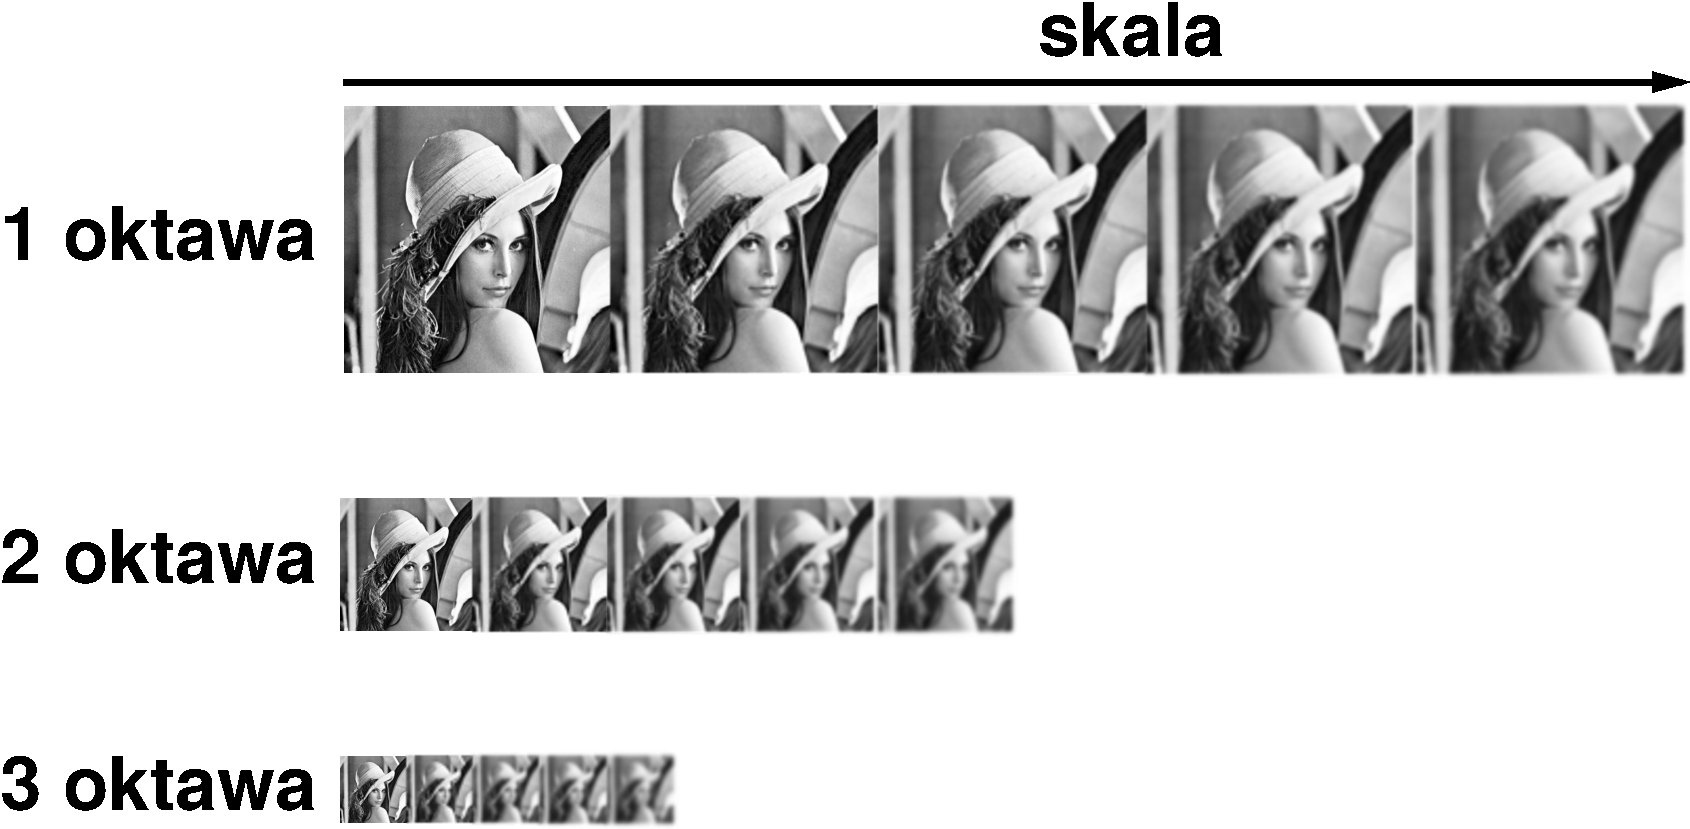
\includegraphics[width=10cm]{gfx/scale_space}
  \caption{Przestrzeń \textit{scale-space} dla przykładowego obrazu. Skala rośnie wraz z siłą filtru Gaussa. Obrazy tej samej wielkości tworzą oktawę.}
  \label{fig:proponowane_algorytmy:scale_space_fig}
\end{figure}

Autor algorytmu SIFT zalecana użycie czterech oktaw i pięciu poziomów siły filtru Gaussa.

\subsubsection{2. Obliczenie \textit{difference of Gaussians}}
\label{sec:proponowane_algorytmy:difference}

Charakterystycznymi punktami obrazu są krawędzie i rogi. Są to miejsca, które najlepiej nadają się na znalezienie cech. Operacja \textit{laplacian of Gaussian, LoG} świetnie sobie radzi w wykrywaniu krawędzi i rogów w obrazie. Polega ona na wyeliminowaniu szumu poprzez zaaplikowanie filtru Gaussa, a następnie obliczenie drugiej pochodnej. Na rysunku \ref{fig:proponowane_algorytmy:gauss} przedstawione jest działanie LoG na jednowymiarowym fragmencie obrazu.

\begin{figure}[H]
  \centering
  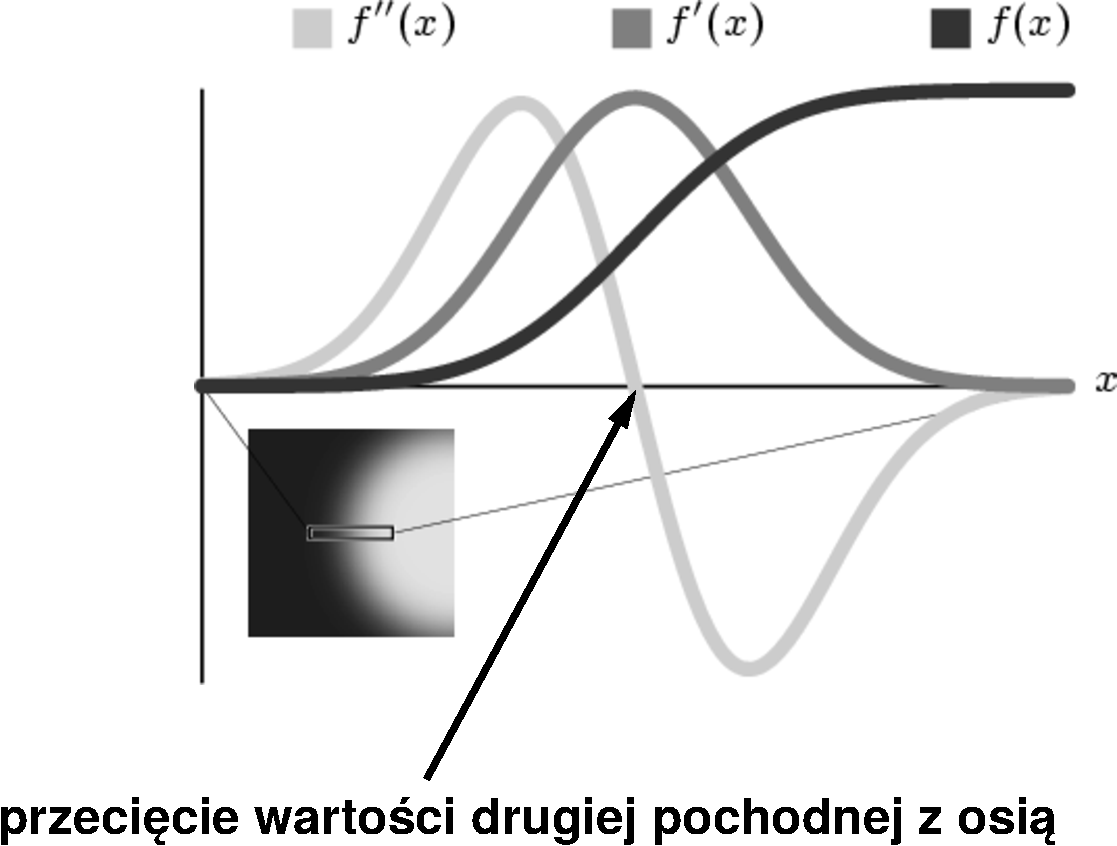
\includegraphics[width=8cm]{gfx/gauss}
  \caption{Przykład wykrycia krawędzi przez LoG. Czarny wykres przedstawia jednowymiarowy sygnał z obrazu. Miejsce przecięcia się z osią drugiej pochodnej tzw. \textit{zero-crossing} wskazuje miejsce krawędzi w oryginalnym obrazie.}
  \label{fig:proponowane_algorytmy:gauss}
\end{figure}

Obliczenie drugiej pochodnej całego obrazu jest natomiast kosztownym procesem. SIFT implementuje operację \textit{difference of Gaussians, DoG}, która w przybliżeniu jest równa LoG, ale jest o wiele szybsza. DoG polega na odjęciu dwóch kolejnych obrazów z tej samej oktawy. Rysunek \ref{fig:proponowane_algorytmy:dog} przedstawia operację DoG. DoG jest obliczane dla każdej pary w każdej oktawie.

\begin{figure}[htb]
  \centering
  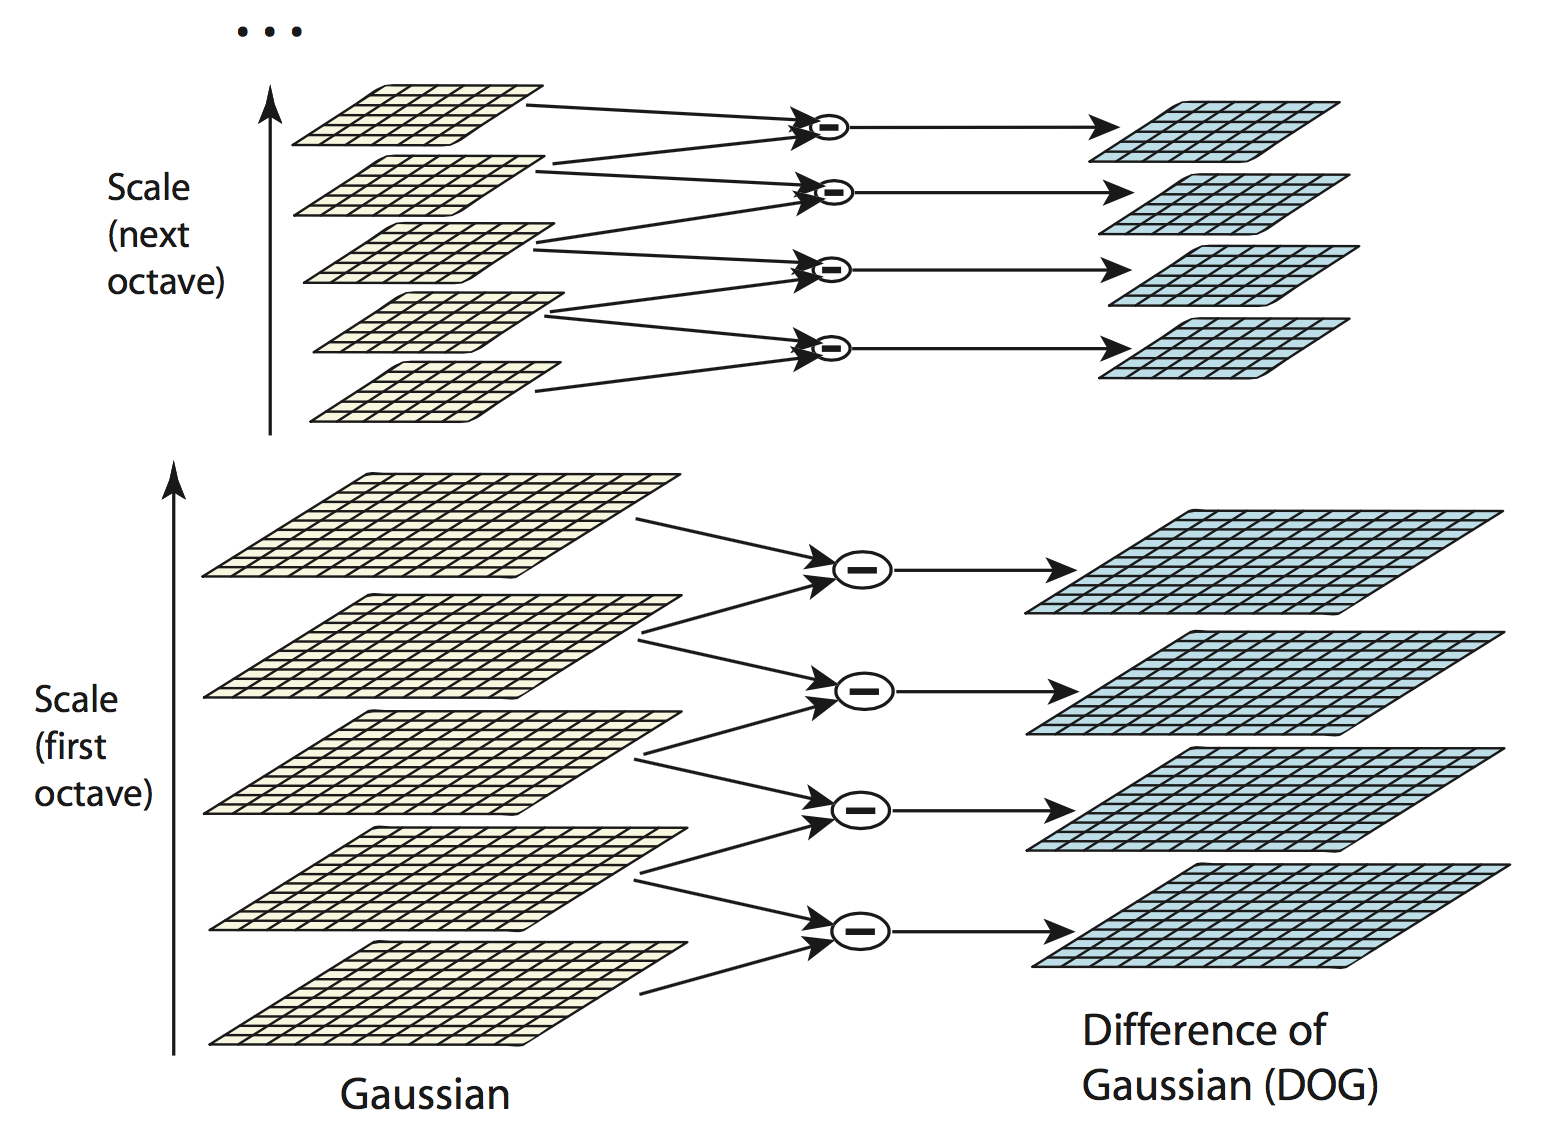
\includegraphics[width=10cm]{gfx/dog}
  \caption{\cite{Lowe:2004:DIF:993451.996342} Poprzez proces odjęcia kolejnych zdjęć z jednej oktawy otrzymujemy obrazy DoG, które doskonale odzwierciedlają LoG.}
  \label{fig:proponowane_algorytmy:dog}
\end{figure}

\subsubsection{3. Ekstrakcja cech}
\label{sec:proponowane_algorytmy:ekstrakcja_cech}

Następnym krokiem po obliczeniu obrazów DoG jest ekstrakcja cech. Na rysunku \ref{fig:proponowane_algorytmy:dog} druga pochodna poprzez przecięcie osi (\textit{zero-crossing}) wskazuje miejsce występowania krawędzi w oryginalnym obrazie, natomiast można też zauważyć, że lokalne maksimum z lewej strony i lokalne minimum z prawej strony wykresu wskazują dwie strony krawędzi. SIFT ekstrahuje cechy poprzez wykrycie lokalnych maksimów i minimów w obrazach DoG. Proces wyjaśniony jest na rysunku \ref{fig:proponowane_algorytmy:max}.

\begin{figure}[H]
  \centering
  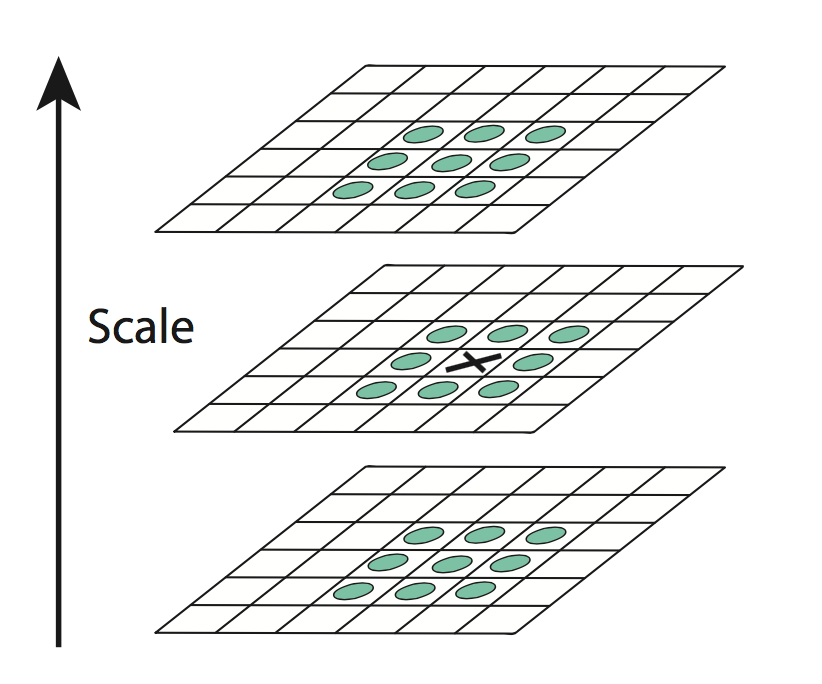
\includegraphics[width=6cm]{gfx/max}
  \caption{\cite{Lowe:2004:DIF:993451.996342} Maksima i minima wykrywane są za pomocą porównania wartości aktualnie badanego piksela (zaznaczony czarnym krzyżykiem) z jego 26 sąsiadami powstałymi poprzez złączenie kolejnych obrazów DoG z jednej oktawy. Cecha jest wykrywana w miejscu aktualnie badanego piksela jeżeli wartość tego piksela jest największa lub najmniejsza spośród 26 sąsiadów.}
  \label{fig:proponowane_algorytmy:max}
\end{figure}

\subsubsection{4. Filtrowanie cech}
\label{sec:proponowane_algorytmy:filtracja_cech}

W większości przypadków ekstrakcja cech może wygenerować ich ogromną ilość. SIFT poprzez zastosowanie następujących dwóch filtrów pozbywa się cech najgorszej jakości:

\begin{enumerate}
\item Pierwszy filtr polega na sprawdzeniu intensywności piksela obrazu DoG w miejscu gdzie wykryto cechę. Jeżeli wartość piksela jest mniejsza niż ustalony wcześniej próg cecha jest odrzucana.
\item Drugi filtr polega na obliczeniu dwóch prostopadłych do siebie gradientów w miejscu wystąpienia cechy. W zależności od otoczenia cechy możliwe są 3 opcje:
  \begin{itemize}
  \item Wartości dwóch gradientów będą małe z czego wynika, że w otoczeniu cechy jest region płaski. Cecha jest odrzucana.
  \item Wartość jednego gradientu będzie duża, a drugiego mała. Oznacza to, że wzdłuż gradientu z małą wartością występuje krawędź w oryginalnym obrazie (gradient z dużą wartością jest prostopadły do krawędzi). Cecha jest odrzucana.
  \item Wartość dwóch gradientów będzie duża. Oznacza to, że w cecha znajduje się w miejscu występowania rogu w oryginalnym obrazie. Cecha jest zachowana ze względu na to, że rogi są najlepszymi cechami.
  \end{itemize}
\end{enumerate}

\subsubsection{5. Przydzielenie orientacji cechom}
\label{sec:proponowane_algorytmy:orientacja}

Kolejny krok algorytmu SIFT polega na obliczeniu orientacji każdej cechy na podstawie jej otoczenia, przez co deskryptory cech mogą być przedstawione względnie do swojej orientacji. Dzięki temu algorytm SIFT jest niezależny od rotacji obrazów. Proces obliczenia orientacji zaczyna się od wyznaczenia wartości gradientu $m(x, y)$ i orientacji $\theta(x, y)$ dla każdego piksela z otoczenia wokół cechy za pomocą wzorów:

\begin{equation}
m(x, y) = \sqrt{(L(x + 1, y) - L(x - 1, y))^2 + (L(x, y + 1) - L(x, y - 1))^2} \\
\label{eq:magnitude}
\end{equation}
\begin{equation}
\theta(x, y) = \tan^{-1}((L(x, y + 1) - L(x, y - 1))/(L(x + 1, y) - L(x - 1, y)))
\label{eq:orientation}
\end{equation}

Następnie na podstawie wartości orientacji tworzony jest histogram, który posiada 36 przedziałów przez co pokrywa zakres orientacji od 0 do 360 stopni. Każdy piksel dodany do histogramu jest ważony poprzez użycie jego wartości gradientu i wartości okrągłego okna filtra Gaussa (piksele znajdujące się dalej od cechy mają mniejszą ważność niż te znajdujące się bliżej). Orientacja odpowiadająca najwyższej wartości w histogramie jest wybrana jako orientacja cechy. Dodatkowo każda orientacja, która posiada wartość większą niż 80\% maksymalnej wartości w histogramie jest zapisywana jako nowa cecha obrazu.

\subsubsection{6. Generacja deskryptorów cech}
\label{sec:proponowane_algorytmy:deskryptor}

Deskryptor cechy musi ją charakterystycznie określać i być łatwy do obliczenia. SIFT przedstawia cechę jako 128 elementowy wektor, który został stworzony poprzez wykonanie następujących kroków:

\begin{enumerate}
\item Tworzone jest otoczenie 16 na 16 pikseli wokół cechy.
\item Dla każdego piksela w otoczeniu cechy jest liczona wartość gradientu oraz orientacja zgodnie ze wzorami \ref{eq:magnitude} i \ref{eq:orientation}. Każdą orientację piksela w otoczeniu odejmujemy od orientacji cechy obliczonej w poprzednim punkcie, przez co algorytm SIFT jest niezależny od rotacji obrazu.
\item Wartości gradientu oraz orientacji są ważone przez okrągłe okno filtru Gaussa i są następnie gromadzone poprzez utworzenie histogramu orientacji, który określa informacje w regionach 4 na 4 piksele. Rysunek \ref{fig:proponowane_algorytmy:descriptor} przedstawia proces kumulacji wartości gradientu oraz orientacji poprzez wykorzystanie histogramu.
\begin{figure}[H]
  \centering
  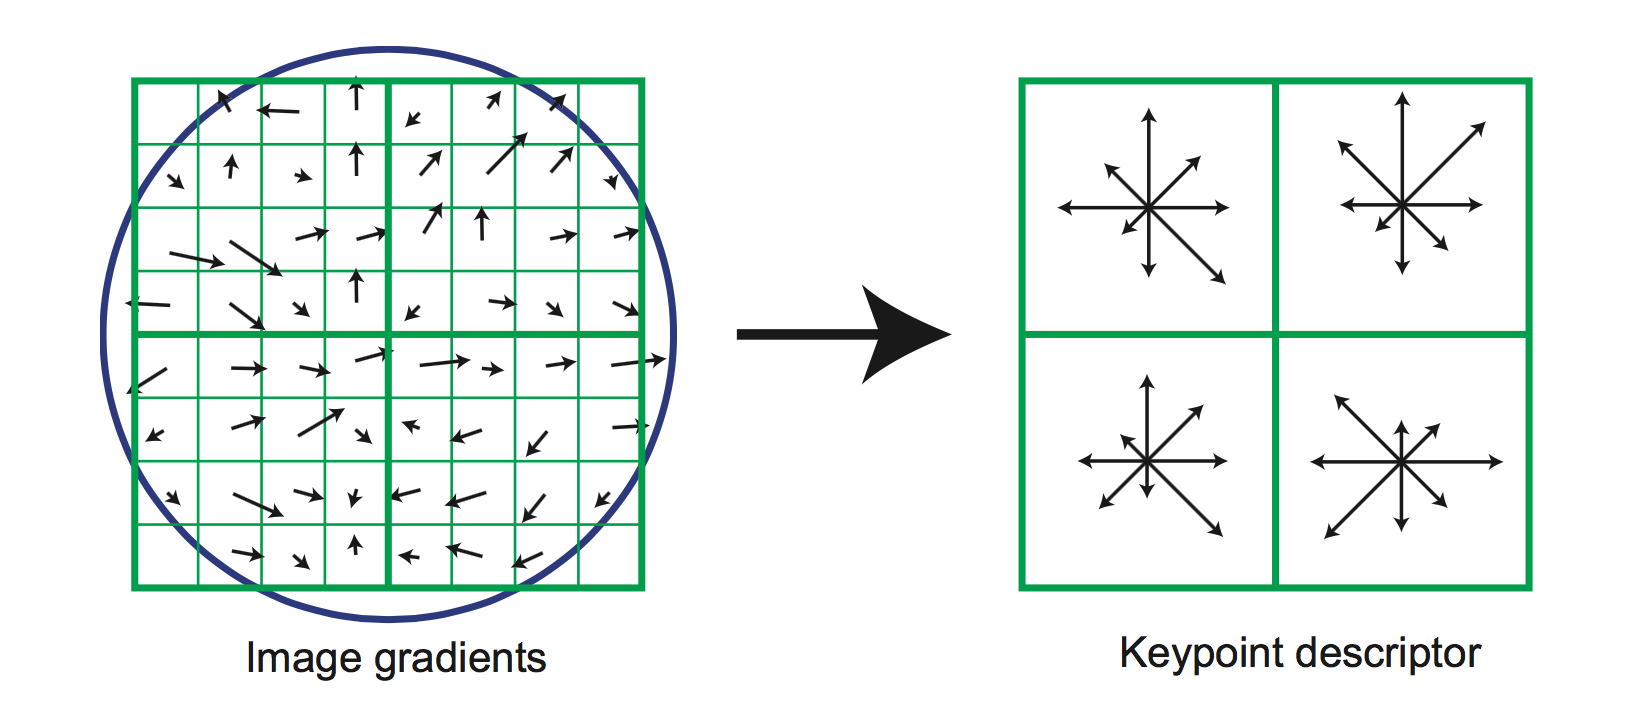
\includegraphics[width=\textwidth]{gfx/descriptor}
  \caption{\cite{Lowe:2004:DIF:993451.996342} \textbf{Lewy obraz:} Wartości orientacji oraz gradientu z uwzględnieniem okrągłego okna filtru Gaussa. \textbf{Prawy obraz:} Wartości z obszarów 4 na 4 piksele są gromadzone w histogramie, który posiada 8 przedziałów. Wartości orientacji z lewego obrazu, które wchodzą do jednego przedziału histogramu są sumowane (np. piksel z orientacją 12 stopni wchodzi do przedziału 0 - 44 stopni histogramu i jego wartość jest dodawana z każdą orientacją 0 - 44 stopni).}
  \label{fig:proponowane_algorytmy:descriptor}
\end{figure}
\item Prawy obraz z rysunku \ref{fig:proponowane_algorytmy:descriptor} przedstawia deskryptor z obszaru 8 na 8 pikseli, który posiada 32 elementy (4 obszary, każdy posiada 8 orientacji). Autor algorytmu SIFT podaje, że najlepsze rezultaty można uzyskać poprzez policzenie deskryptora z obszaru 16 na 16 pikseli wokół cechy, wtedy deskryptor posiada 128 elementów (16 obszarów, każdy posiada 8 orientacji).
\item Na koniec 128 elementowy wektor jest normalizowany.
\end{enumerate}

\subsubsection{Sposób wykorzystania algorytmu SIFT w programie}
\label{sec:proponowane_algorytmy:sift_wykorzystanie}

Biblioteka OpenCV posiada zaimplementowany algorytm SIFT i jego użycie sprowadza się do paru linii kodu:

\begin{verbatim}
SIFT featuresFinder = SIFT::SIFT(...);
featuresFinder(...);
\end{verbatim}

Konstruktor \texttt{SIFT::SIFT(...)} tworzy nam obiekt \texttt{SIFT}, który posiada funkcjonalność algorytmu SIFT. Do konstruktora \texttt{SIFT::SIFT(...)} podajemy parametry algorytmu tj. ilość najlepszych cech do zwrócenia, ilość oktaw do wykorzystania, progi do filtrowania wykrytych cech (sekcja \ref{sec:proponowane_algorytmy:filtracja_cech}) oraz siłę filtru Gaussa. Operator \texttt{featuresFinder(...)} przyjmuje obraz w którym mają zostać znalezione cechy i zwraca miejsca wystąpienia tych cech oraz ich deskryptory.

\subsection{Dopasowanie wyekstrahowanych cech}
\label{sec:proponowane_algorytmy:dopasowanie}

\subsection{Filtrowanie dopasowań}
\label{sec:proponowane_algorytmy:filtrowanie}

\subsubsection{Filtrowanie na podstawie wiedzy dziedzinowej}
\label{sec:proponowane_algorytmy:filtrowanie_dziedzinowe}

\subsubsection{RANSAC}
\label{sec:proponowane_algorytmy:ransac}

\section{Rejestracja kafelków poprzez wykrycie położeń naczyń krwionośnych w kafelkach}
\label{sec:proponowane_algorytmy:depth_first_search}

\section{Estymacja macierzy transformacji pomiędzy kafelkami}
\label{sec:proponowane_algorytmy:estymacja}

\section{Globalna rejestracja kafelków}
\label{sec:proponowane_algorytmy:globalna_rejestracja}

\section{Łączenie kafelków}
\label{sec:proponowane_algorytmy:laczenie_kafelkow}
